\documentclass[tikz,border=5pt]{standalone}
\usepackage[UTF8]{ctex}
\usepackage{amsmath,amssymb}
\usetikzlibrary{arrows.meta,calc}
\tikzset{>=Stealth,line cap=round,line join=round,
electric/.style={red!75!black,thick},
magnetic/.style={blue!75!black,thick},
aux/.style={gray!70,dashed,thin}}
\begin{document}
% 1. Open cylindrical shell: ellipses are perspective circles, not extra discs.
\begin{tikzpicture}[font=\small,scale=1]
\fill[blue!4](-1.65,-2)--(-1.65,2)
arc(180:360:1.65 and .48)--(1.65,-2)
arc(0:-180:1.65 and .48)--cycle;
\draw[aux](-1.65,2)arc(180:0:1.65 and .48);
\draw[thick](-1.65,2)arc(180:360:1.65 and .48);
\draw[aux](-1.65,-2)arc(180:0:1.65 and .48);
\draw[thick](-1.65,-2)arc(180:360:1.65 and .48);
\draw[thick](-1.65,-2)--(-1.65,2);
\draw[thick](1.65,-2)--(1.65,2);
\draw[aux](0,-2.8)--(0,2.9);
\draw[->](0,2.9)--(0,3.6)node[above]{$z$};
\fill(0,2)circle(1.2pt);
\draw[magnetic,->](0,2)--(1.65,2)node[midway,above=2pt]{$r$};
\draw[magnetic,->](-.80,3.05)arc(180:350:.80 and .23);
\node[blue!75!black]at(1.12,3.07){$\omega$};
\draw[thin](1.25,.55)--(2.15,.90);
\node[anchor=west,align=left]at(2.20,.90){$\sigma$：面电荷密度\\$\mu$：总面质量密度};
\end{tikzpicture}
% 2. Cross sections viewed from +z. K is azimuthal, B axial.
\begin{tikzpicture}[font=\small]
\begin{scope}
\fill[gray!5](0,0)circle(1.3);
\draw[thick](0,0)circle(1.3);
\foreach \ang in {0,45,90,135,180,225,270,315}{
\draw[electric,->]({1.36*cos(\ang)},{1.36*sin(\ang)})
--({1.95*cos(\ang)},{1.95*sin(\ang)});
}
\node at(0,0){$\mathbf E_{\text{内}}=0$};
\node at(0,-2.55){$\mathbf E_{\text{外}}=\dfrac{\sigma}{\varepsilon_0}\mathbf e_r$};
\node at(0,2.50){电场};
\end{scope}
\begin{scope}[xshift=5.5cm]
\fill[blue!5](0,0)circle(1.3);
\draw[thick](0,0)circle(1.3);
\draw[magnetic,->](1.3,0)arc(0:100:1.3);
\draw[magnetic,->](-1.3,0)arc(180:280:1.3);
\node[blue!75!black]at(1.62,.9){$\mathbf K$};
\node[blue!75!black,font=\Large]at(0,.24){$\odot$};
\node at(0,-.38){$\mathbf B_{\text{内}}$};
\node at(2.00,-.80){$\mathbf B_{\text{外}}=0$};
\node at(0,-2.55){$\mathbf B_{\text{内}}=\mu_0\sigma\omega r\,\mathbf e_z$};
\node at(0,2.50){面电流与磁场};
\end{scope}
\node[gray!70!black]at(2.75,3.08){从 $+z$ 看，图示取 $\sigma>0,\ \omega>0$};
\end{tikzpicture}
% 3. Local wall section: total fields on each side, not self-force fields.
\begin{tikzpicture}[font=\small]
\begin{scope}
\fill[gray!18](-.07,-1.15)rectangle(.07,1.15);
\draw[thick](0,-1.15)--(0,1.15);
\node at(-.95,1.58){筒内};
\node at(.95,1.58){筒外};
\node at(-1.0,.16){$E_{\text{内}}=0$};
\draw[electric,->](.28,.16)--(1.68,.16);
\node[red!75!black]at(1.0,.67){$E_{\text{外}}=\dfrac{\sigma}{\varepsilon_0}$};
\draw[->](.25,-1.38)--(1.2,-1.38)node[right]{$\mathbf e_r$};
\node at(0,-2.15){$\mathbf E_{\text{有效}}=\dfrac{\sigma}{2\varepsilon_0}\mathbf e_r$};
\node at(0,2.13){电场};
\end{scope}
\begin{scope}[xshift=5.65cm]
\fill[gray!18](-.07,-1.15)rectangle(.07,1.15);
\draw[thick](0,-1.15)--(0,1.15);
\node at(-.95,1.58){筒内};
\node at(.95,1.58){筒外};
\draw[magnetic,->](-.87,-.62)--(-.87,.72);
\node[anchor=east]at(-1.02,.12){$B_{\text{内}}=\mu_0K$};
\node at(1.0,.16){$B_{\text{外}}=0$};
\node[blue!75!black,fill=white,inner sep=1pt]at(0,-.40){$\otimes\,K$};
\draw[->](.25,-1.38)--(1.2,-1.38)node[right]{$\mathbf e_r$};
\node at(0,-2.15){$\mathbf B_{\text{有效}}=\dfrac{\mu_0K}{2}\mathbf e_z$};
\node at(0,2.13){磁场};
\end{scope}
\node[gray!70!black]at(2.8,2.77){局部截面；$\mathbf e_z$ 向上，$\mathbf e_\varphi$ 朝纸内};
\end{tikzpicture}
% 4. A finite sector: tangent edge forces and radial distributed pressure.
\begin{tikzpicture}[font=\small,scale=1.1]
\def\RR{2.45}
\def\AA{28}
\coordinate(O)at(0,0);
\coordinate(U)at({\RR*cos(\AA)},{\RR*sin(\AA)});
\coordinate(L)at({\RR*cos(\AA)},{-\RR*sin(\AA)});
\draw[gray!40](O)circle(\RR);
\fill[blue!5](O)--(L)arc(-\AA:\AA:\RR)--cycle;
\draw[blue!65!black,very thick](L)arc(-\AA:\AA:\RR);
\draw[aux](O)--(U);
\draw[aux](O)--(L);
\draw[->](-.35,0)--(3.65,0)node[right]{$x$};
\draw[->](O)--(0,2.85)node[above]{$y$};
\fill(O)circle(1.4pt)node[below left]{$O$};
\draw(.68,0)arc(0:\AA:.68);
\draw(.68,0)arc(0:-\AA:.68);
\node at(.94,.23){$\alpha$};
\node at(.94,-.23){$\alpha$};
\node[rotate=28,fill=white,inner sep=1pt]at(1.5,.81){$r$};
\draw[magnetic,->](U)--++({-1.35*sin(\AA)},{1.35*cos(\AA)})
node[above left]{$T h$};
\draw[magnetic,->](L)--++({-1.35*sin(\AA)},{-1.35*cos(\AA)})
node[below left]{$T h$};
\foreach \psi in {-18,-6,18}{
\draw[electric,->]({\RR*cos(\psi)},{\RR*sin(\psi)})
--({(\RR+.62)*cos(\psi)},{(\RR+.62)*sin(\psi)});
}
\node[red!75!black,anchor=west]at(3.07,1.10){$p_E+p_B$};
\node at(1.05,-3.05){壁带轴向长 $h$；张力沿两端切线};
\end{tikzpicture}
% 5. T is affine in Omega=omega^2, with static intercept.
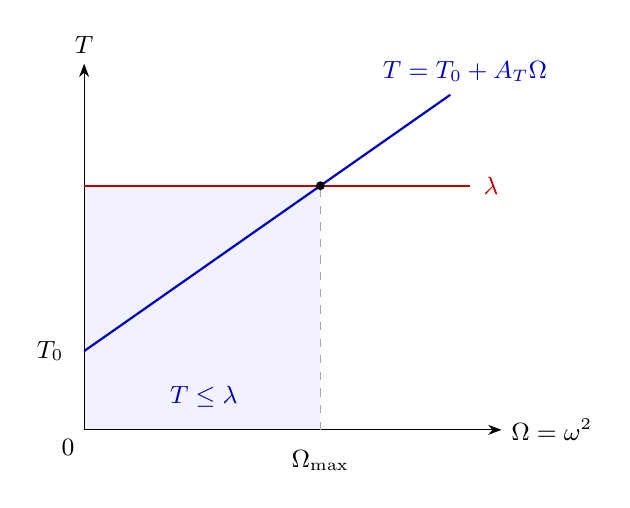
\begin{tikzpicture}[font=\small,x=1cm,y=1cm]
\fill[blue!5](0,0)rectangle(3.0,3.1);
\draw[->](0,0)--(5.3,0)node[right]{$\Omega=\omega^2$};
\draw[->](0,0)--(0,4.65)node[above]{$T$};
\draw[electric](0,3.1)--(4.9,3.1);
\node[red!75!black,anchor=west]at(4.95,3.1){$\lambda$};
\draw[magnetic](0,1)--(4.65,4.255);
\node[blue!75!black,anchor=west]at(3.67,4.55){$T=T_0+A_T\Omega$};
\draw[aux](3.0,0)--(3.0,3.1);
\fill(3.0,3.1)circle(1.6pt);
\node[anchor=east]at(-.14,1){$T_0$};
\node[below=4pt]at(3.0,0){$\Omega_{\max}$};
\node[below left]at(0,0){$0$};
\node[blue!70!black]at(1.52,.42){$T\le\lambda$};
\end{tikzpicture}
\end{document}
